\section{Planteamiento del Problema} \label{problem_statement}

% Este párrafo está cubierto en los antecedentes sobre el e-government
Gobiernos de todo el mundo buscan digitalizar sus
procesos para facilitar la interacción con la población y aumentar la eficiencia
de los mismos, apuntando a lo que la CEPAL llama Gobiernos Digitales y Gobiernos
Inteligentes.

% Tal vez de aquí podemos dejar la especificación de ciertas funcionalidades del trámite
Dentro de todos los procesos administrativos la figura de trámite y el
seguimiento del mismo se encuentra siempre presente a todo nivel y suele ser
motivo o parte del motivo de la creación de muchos sistemas de software
gubernamentales.

El desarrollo de sistemas de software es un proceso largo que requiere por sí
mismo la toma de varias decisiones profesionales para brindar a los usuarios el
mejor producto en el menor tiempo posible y garantizando que se cumplan ciertos
requerimientos funcionales y no funcionales, implicando una gran complejidad que
sería limitante si no fuera por algunas buenas prácticas de desarrollo.

% Esto dedbe ir a los antecedentes
A menudo, los equipos de desarrollo, para evitar que la complejidad de los
sistemas sea excesiva, buscan herramientas de terceros que les permiten no
reinventar la rueda. Estas herramientas, llamadas paquetes de software, que
pueden ser librerías o incluso \textit{frameworks} de desarrollo, ofrecen una serie de
ventajas a los proyectos de desarrollo, así como algunas limitaciones que, en la
mayoría de los casos, y dependiendo del proyecto, no son relevantes, pero
requieren la atención del equipo de profesionales.

Estas herramientas, que forman parte fundamental del desarrollo moderno, suelen
ser de código abierto, o al menos así se prefieren por muchos profesionales,
dadas sus ventajas de seguridad y versatilidad.

Es importante notar también que en algunos países se demanda o prefiere el uso
de software libre en el ámbito público. Tal es el caso de Bolivia, que en su
artículo 77 de la ley general de telecomunicaciones, tecnologías de información
y comunicación indica que se debe promover y priorizar el uso del mismo dentro
de los órganos ejecutivo, legislativo, judicial y electoral.
% Hasta acá se va a antecedentes

% Parte de esto debe ir a state of the art
Por lo anteriormente descrito podemos encontrar una gran cantidad de tecnologías
abiertas usadas para el desarrollo de sistemas, como la librería Carbon de PHP,
el estándar \textit{EcmaScript} o el popular \textit{framework} de desarrollo \textit{Laravel}, las cuales,
a pesar de proporcionar utilidades que facilitan la creación de proyectos
pequeños y medianos de software, no proporcionan de manera específica un marco
de trabajo confiable y específico para trabajar con los tan frecuentes trámites
administrativos y su seguimiento, obligando a los desarrolladores a reinventar
la rueda en cada proyecto de este tipo.

El caso que se toma para este proyecto, que es el sistema SIAI del
Viceministerio de Desarrollo Productivo, desarrollado por la empresa 2IES, tiene
un módulo de seguimiento de trámites realizado desde cero para el mismo y,
además de ser en el que se basará este proyecto y sobre el cual se aplicará para
medir el éxito del mismo, es un claro ejemplo de la necesidad de un paquete
reutilizable para la creación de módulos de trámites y seguimiento de trámites.

Otros sistemas, cuyo código fuente, se escapan al conocimiento del autor de este
documento, pero que se estima requirieron un desarrollo desde cero para su
módulo de trámites son:

\begin{itemize}
    \item Sistema de Matriculación de la UMSA

    \item Sistema para permisos de vidrios polarizados

    \item Sistema para permisos de circulación en pandemia

    \item Procedimiento para autorización de vidrios oscurecidos
\end{itemize}

\begin{figure}[!htpb]
    \centering
    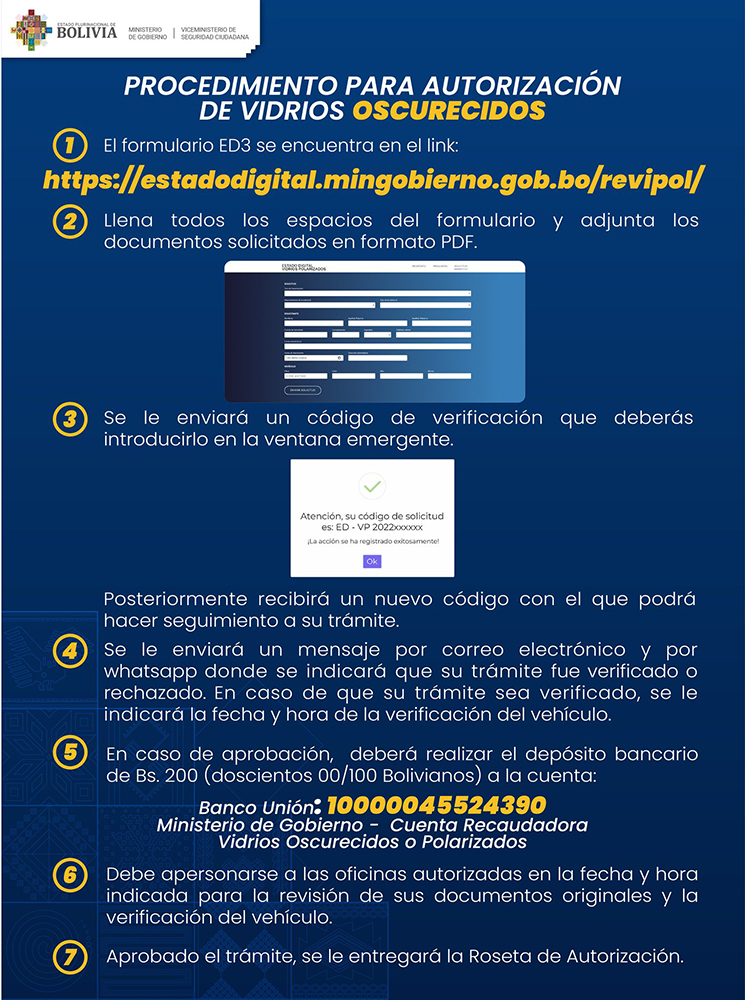
\includegraphics[width=0.6\textwidth]{assets/tramiteoscurecidos.jpg}
    \caption{Pasos del trámite para vidrios oscurecidos que se realizó en línea}
    \label{fig:polarized_procedure_steps}
\end{figure}

Entre los sistemas anteriormente expuestos, se hace énfasis en los sistemas
creados en época de pandemia, o el caso de los vidrios oscurecidos de la figura
\ref{fig:polarized_procedure_steps} , los cuales debían ser desarrollados con
premura dadas las circunstancias, lo cual puede ser facilitado con una librería
de software.

La carencia de una librería específica a los trámites y su seguimiento hacen
visibles varias desventajas:

\begin{itemize}
    \item Reinvención de la rueda en varios proyectos de características
          similares.

    \item Poca atención al detalle para un módulo de gran importancia.

    \item Tiempos de desarrollo mayores.

    \item Mayor coste.

    \item Sobre-ingeniería en proyectos pequeños.

    \item Menor adopción de sistemas digitales en el aparato público.

    \item Mayor susceptibilidad a desarrollos fallidos.

    \item Falta de características.

    \item Dificultad mayor en la redacción de la documentación.

    \item Poca presencia de proyectos \textit{open source} bolivianos.
\end{itemize}

Actualmente existen librerías que ayudan con un concepto muy útil en el
seguimiento de trámites que son las máquinas de estados. Sin embargo, no son
específicas, son poco usadas y carecen de una buena documentación o facilidades
para el desarrollador.

Además, sistemas similares a los de seguimientos de trámite también existen en
el mercado, pero como productos cerrados y genéricos que no garantizan seguridad
para un sistema gubernamental y no pueden ser reutilizados por varios proyectos
de forma gratuita como es el caso de una librería de código abierto.

Por lo expuesto, se tiene una visión inicial que consiste en la premisa de que
cuando una funcionalidad es común en distintos sistemas, una solución viable y
común es la creación de una herramienta reutilizable de código abierto que ayude
en su implementación. Esto proporciona varias ventajas y se suscribe al
principio DRY \brackettext{\textit{Don't repeat yourself}} y al primer principio \textit{SOLID}
sobre la \textit{single responsibility}.

Sin embargo, una librería \textit{open source} acarrea varios desafíos en su realización,
muchos de ellos académicos, de los cuales a continuación se listan algunos:

\begin{itemize}

	\item Elección de un entorno sobre el cual aplicar este proyecto: Una
	      librería puede estar limitada a un lenguaje de programación o incluso a
	      un marco de desarrollo. Esta decisión es importante tomarla al inicio
	      del proyecto.

	\item Metodología de desarrollo: Adoptar una buena metodología es importante
	      en una librería, ya que ésta será utilizada por muchos proyectos que
	      confiaran en la misma. Además, al ser \textit{open source}, se espera que de
	      tener éxito la misma siga mejorando.

	\item Arquitectura de Software: Este es un tema muy someramente estudiado
	      durante el transcurso de la carrera de ingeniería Electrónica de la
	      UMSA, pero es muy necesario para tomar las mejores decisiones en el
	      desarrollo de un sistema.

	\item Documentación: Escribir la documentación de una librería que se espera
	      sea utilizada por muchas personas es de mayor relevancia. Se requiere un
	      buen lenguaje técnico y habilidades de redacción, pero a la vez la
	      capacidad para que lo descrito sea fácil de entender por la mayor
	      cantidad de personas.

	\item \textit{Knowhow open source}: Se cuenta con muy poco conocimiento del
	      desarrollo de software libre en el contexto local y mucho menos de
	      sistemas con éxito.

	\item Versionado: Cualquier proyecto de software moderno requiere el uso de
	      sistemas de versionado, pero en un proyecto de código abierto esto es
	      especialmente importante para permitir colaboraciones externas.

	\item Buenas prácticas de desarrollo y uso de patrones de diseño: Para tener
	      una buena librería existen libros de recomendaciones y patrones que
	      pueden ser empleados, además de experiencias compartidas en internet por
	      distintos desarrolladores.  Las mismas pueden potenciar un proyecto y
	      son importantes de aprender.

	\item Infraestructura y escalabilidad: La librería debe ser pensada para
	      poder ser desplegada en sistemas grandes y poder ser escalable. El tema
	      de escalabilidad es en sí mismo un campo de estudio dentro del
	      despliegue de sistemas.

	\item Testabilidad: Los proyectos de software moderno tienen como proceso
	      importante el del testing, el cual permite realizar desarrollos que cumplan con
	      lo que se desea en su diseño y que no hagan algo distinto \parencite{myersArtSoftwareTesting2012}.
	      Sin embargo, el campo del \textit{testing} no es ni minimamente explorado en
	      instituciones universitarias, a pesar de su importancia.
\end{itemize}